\chapter{Data Structures}

Simply put, a \textbf{data structure} is a way of organizing data in a structured way so that it can be processed efficiently. In the context of programming contests, this data generally consists of integers, and in some cases, floating point numbers and strings. Good knowledge of data structures is essential to being able to solve certain problems efficiently.

In all likelihood, you won't ever have to code elementary data structures because the standard libraries of most programming languages already include implementations of them. However, it's important to understand how data structures work so you understand their performance characteristics and can decide which one will work best in a given situation. Understanding how simple data structures work will also help you when you need to write more complex data structures on your own.



\section{Lists}

A \textbf{list} represents a sequence of ordered elements. The elements are ordered in the sense that each is associated with an \textit{index} that represents its position in the list. The main operations that we'd like to perform on a list are accessing the item at some position, and adding or removing an element at some position.


\subsection{Arrays}

Arrays are a fundamental type of data structure, implemented at the language level, that can be used as a list. Because they are created by requesting a block of memory from the operating system, one limitation of arrays is that they must have a \textit{fixed size}. A good property of arrays, on the other hand, is that we can access any element of an array in $O(1)$ time, because of their low-level nature.

\subsection{Dynamic arrays} \label{sec:dynamic-array}

\begin{figure}
\centering
{
\begin{tikzpicture}[
  thick,
  myrect/.style={
    draw,
    fill=myseagreen,
    rectangle split,
    rectangle split horizontal,
    rectangle split parts=#1,
    rectangle split part align=left,
    text width=5ex,
    text centered
    },
  mycallout/.style={
    shape=rectangle callout,
    rounded corners,
    fill=mysalmon,
    callout absolute pointer={#1},
    callout pointer width=1cm
  }  
]

\node[myrect=3]
  (array1)
  {
  					\strut \texttt{"a"}
  \nodepart{two}	\strut \texttt{"b"}
  \nodepart{three}	\strut \texttt{null}
  };
\foreach \Valor [count=\Valori from 0] in {one ,two ,three }
  \node[below] at (array1.\Valor south) {\Valori};

\node[myrect=3]
  (array2)[below=of array1]
  {
  					\strut \texttt{"a"}
  \nodepart{two}	\strut \texttt{"b"}
  \nodepart{three}	\strut \texttt{"c"}
  };
\foreach \Valor [count=\Valori from 0] in {one ,two ,three }
  \node[below] at (array2.\Valor south) {\Valori};

\node[myrect=6]
  (array3)[below=of array2]
  {
  					\strut \texttt{"a"}
  \nodepart{two}	\strut \texttt{"b"}
  \nodepart{three}	\strut \texttt{"c"}
  \nodepart{four}	\strut \texttt{null}
  \nodepart{five}	\strut \texttt{null}
  \nodepart{six}	\strut \texttt{null}
  };
\foreach \Valor [count=\Valori from 0] in {one ,two ,three , four , five , six }
  \node[below] at (array3.\Valor south) {\Valori};

\node[myrect=6]
  (array4)[below=of array3]
  {
  					\strut \texttt{"a"}
  \nodepart{two}	\strut \texttt{"b"}
  \nodepart{three}	\strut \texttt{"c"}
  \nodepart{four}	\strut \texttt{"d"}
  \nodepart{five}	\strut \texttt{null}
  \nodepart{six}	\strut \texttt{null}
  };
\foreach \Valor [count=\Valori from 0] in {one ,two ,three , four , five , six }
  \node[below] at (array4.\Valor south) {\Valori};

\end{tikzpicture}
}
\caption{Inserting two elements into a dynamic array of size two.}
\end{figure}


A major caveat to arrays is their \textit{fixed size}, which means that we need to know the maximum number of elements we'll have in an array before we create it. If we need to append an element beyond the capacity we've allocated, we're out of luck. The solution to this is pretty simple: we can simply create a larger array, and copy the elements over.

A \textbf{dynamic array}, or a resizable array, provides an abstraction over this process. It maintains a \textit{backing array} that stores the actual elements. When an insertion is impossible because there's not enough space, it "resizes" itself by creating a new backing array of a larger size, copying the elements over, then discarding the old backing array.

When we do need to resize our array, we'll typically create a backing array of \textit{two times the size} of the previous one. This means that we'll take up more space than strictly necessary: half of the indexes in the new array will be null! However, the benefit of this is that we can add more elements without resizing the array again.

When we do have \textit{excess capacity} in our backing array, an insertion operation at the end will only take $O(1)$. Otherwise, we'll need to perform an $O(n)$ resize. However, if we double the size of our backing array every time we resize it, the total complexity over $k$ insertions will be approximately $O(k + \frac{k}{2} + \frac{k}{4} + \dots) = O(k)$. Thus, the \textit{average} time complexity of an insertion operation is $O(1)$. Because the cost of resizing an array is spread out over $k$ operations, we say that the \textbf{amortized} complexity of insertion is $O(1)$.

Because dynamic arrays are backed by arrays, we can access any element in $O(1)$. Inserting and deleting elements at the end is amortized $O(1)$. However, inserting and deleting elements at any position will take $O(N)$, since we'll need to shift all elements that come after the insertion or deletion point by one position.


\subsection{Linked lists}

A \textbf{linked list} data structure represents a list through a series of \textit{nodes}. Each of these nodes is an object that stores the value of the item it represents, and a pointer to the next node. If there are no more items in the list, we typically represent this with a null pointer.

How can we access items in this list? Since each node is only referenced by the previous node in the list, we need to access nodes $0 \dots k-1$ in order to get to item $k$. This is one of the large downsides of linked lists: accessing elements requires linear, not constant time.

A good thing about linked lists, however, is that they lend themselves well to recursion. As with a recursive function, there is a base case --- when the pointer is null --- and otherwise, a recursive case that splits the list into two parts: the current element, and everything else.

\subsubsection{Doubly-linked lists}

\begin{figure}
\centering
\begin{tikzpicture}[
        list/.style={
            very thick, rectangle split, 
            rectangle split parts=3, draw, 
            rectangle split horizontal, minimum size=18pt,
            inner sep=5pt, text=black,
            rectangle split part fill=myseagreen
        }, 
        ->, start chain, very thick
      ]

  \node[list,on chain] (dummy) {\nodepart{second} \texttt{null}};
  \node[list,on chain] (A) {\nodepart{second} \texttt{"a"}};
  \node[list,on chain] (B) {\nodepart{second} \texttt{"b"}};
  \node[list,on chain] (C) {\nodepart{second} \texttt{"c"}};

    \path[*->] let \p1 = (dummy.three), \p2 = (dummy.center) in (\x1,\y2) edge [bend left] ($(A.one)+(0,0.2)$);
  \path[*->] let \p1 = (A.three), \p2 = (A.center) in (\x1,\y2) edge [bend left] ($(B.one)+(0,0.2)$);
  \path[*->] let \p1 = (B.three), \p2 = (B.center) in (\x1,\y2) edge [bend left] ($(C.one)+(0,0.2)$);
  
%  \draw[*->] let \p1 = (C.three), \p2 = (C.center) in (\x1,\y2) -- (dummy);

%  \draw[*->] ($(A.one)+(0.2,0.1)$) -- (dummy);
  \path[*->] ($(B.one)+(0.1,0.1)$) edge [bend left] ($(A.three)+(0,-0.05)$);
  \path[*->] ($(C.one)+(0.1,0.1)$) edge [bend left] ($(B.three)+(0,-0.05)$);
    \path[*->] ($(A.one)+(0.1,0.1)$) edge [bend left] ($(dummy.three)+(0,-0.05)$);
    
    \draw[*->] ($(C.three)+(0.0,0.2)$) -- ($(C.three)+(1.0,0.2)$) -- ($(C.three)+(1.0,-0.8)$) -- ($(dummy.one)+(-0.9,-0.8)$) -- ($(dummy.one)+(-0.9,0.2)$) -- ($(dummy.one)+(0.1,0.2)$);

    \draw[<-*] ($(C.three)+(0.0,0.0)$) -- ($(C.three)+(0.8,0.0)$) -- ($(C.three)+(0.8,-0.6)$) -- ($(dummy.one)+(-0.7,-0.6)$) -- ($(dummy.one)+(-0.7,0.0)$) -- ($(dummy.one)+(0.1,0.0)$);

\end{tikzpicture}
\caption{A doubly-linked list with a dummy node.}
\label{doubly-linked-list}
\end{figure}

Above, we stated that it takes $k$ memory accesses to access item $k$. So the maximum number of memory accesses in a linked list of size $n$ would be $n$, to access $a_{n-1}$. You might notice, however, that if we could start from either end of a linked list, it would only take $1$ step to access element $n-1$! This would halve the maximum number of accesses to $\frac{n}{2}$, to access element $a_{n/2}$.

So far, we've only talked about \textbf{singly-linked lists}, in which each node only has one pointer to the next node. To access nodes in either direction, we need to use \textbf{doubly-linked lists}, in which each node has a pointer to the next \textit{and the previous} nodes. This uses slightly more memory, but is used more frequently because it allows us to easily modify both the front and the back of a linked list.

The easiest way to implement a doubly-linked list is using a cyclical list with a dummy node after the last item and before the first. This makes the code to implement linked lists simpler. Figure \ref{doubly-linked-list} illustrates such a linked list with elements "a", "b", and "c", with the dummy node on the left.


\subsection{Efficiency}

\begin{figure}[b]
\centering
\begin{tabular}{| l | l | l |} \hline
    \textbf{Operation}           & \textbf{Dynamic array}    & \textbf{Linked list}  \\ \hline
    Access front/back   & $O(1)$           & $O(1)$       \\ \hline
    Access position $i$ & $O(1)$           & $O(N)$       \\ \hline
    Add to front        & $O(N)$           & $O(1)$       \\ \hline
    Add to back         & $O(1)$ amortized & $O(1)$       \\ \hline
    Add to position $i$ & $O(N)$           & $O(N)$       \\ \hline
\end{tabular}
\caption{Complexity of various list operations.}
\end{figure}

In general, dynamic arrays are more efficient than linked lists, as their values are stored in contiguous memory, and benefit from CPU caching. However, we might want to use linked lists in certain cases:

\begin{enumerate}
    \item If we often need to insert or delete elements from the front of a list, this will take $O(N)$ time in a dynamic array. We'll address this in section~\ref{sec:deque} when we talk about deques.
    \item Individual insertions at the end of a dynamic array can take up to $O(N)$ time, even if their amortized cost is $O(1)$. In some real-time applications, we'd prefer a linked list, to guarantee $O(1)$ time.
    \item Furthermore, we can join together two linked lists in $O(1)$ time by changing the pointers at the end.
\end{enumerate}


\section{Stacks and Queues}

\subsection{Stacks}

A \textbf{stack} is analogous to how a stack of books would work. Suppose we were creating a stack of books. We might start by putting down book $A$, and then book $B$ on top of it. Then, if we tried to remove a book, we would end up removing book $B$, which is at the top of the stack. Because the the last element added will be the first one removed, stacks are said to operate in \textbf{LIFO} (Last in, First Out) order. We call adding an element a \textit{push} operation, and removing an element a \textit{pop} operation.

With a simple array, we can construct a fixed-size stack relatively simply, even in low-level code: all we have to do is maintain a counter of the number of elements in the stack. We increment the counter to add an element, and decrement it to remove an element. If we use a dynamic array, it can serve as a stack with no size restriction, with insertion and removal in amortized $O(1)$ time.


\subsection{Queues}

A \textbf{queue} operates much like a queue does in real life: imagine waiting in a checkout queue at a grocery store. The first person to get there will, no matter how many people line up behind up them, be the first to be served. In fact, the order of people who arrive in the queue will be the same as the order of people leaving the queue. Therefore, we say that the queue operates in \textbf{FIFO} (first in, first out) order. We call adding an element an \textit{enqueue} operation, and removing an element a \textit{dequeue} operation.


\subsection{Deques} \label{sec:deque}

%One end is the \textit{left}, \textit{front}, \textit{head}, or \textit{first}.
%The other end is the \textit{right}, \textit{back}, \textit{tail}, or \textit{last}.

% https://en.wikipedia.org/wiki/Double-ended_queue
% https://docs.oracle.com/javase/8/docs/api/java/util/Deque.html
% https://docs.python.org/3/library/collections.html#collections.deque
% http://www.cplusplus.com/reference/deque/deque/

A \textbf{deque} (pronounced as \textit{deck}) supports the same operations that a stack and a queue do. As a result, if we have an implementation of a deque, we can use it either as a stack or a queue, depending on whether we want elements in FIFO or LIFO order. 

However, when combining these two interfaces, we run into a problem with our model: what should happen when we interlace stack operations with queue operations? Should a \textit{push} add items at the same place as an \textit{enqueue}, or at the opposite end? Instead, we revert to an abstract data type more similar to that of a list, with a \textit{front} and a \textit{back}. Our goal is to add and remove elements efficiently at either end.

The most straightforward way to implement a deque is to use a \textbf{doubly-linked list}. As we discussed above, this allows us to access, add, or remove elements at either end of a list in $O(1)$ time. Furthermore, although a linked list requires $O(n)$ time to access an arbitrary element, this isn't a downside for implementing a deque.


\section{Trees} \label{sec:trees}

\begin{figure}[h]
\centering
\begin{tikzpicture}[very thick,level/.style={sibling distance=70mm/#1}]
\node [vertex] (r){\texttt{"a"}}
  child {
    node [vertex] {\texttt{"b"}}
    child {
      node [vertex] {\texttt{"d"}}
    }
  }
  child {
    node [vertex] {\texttt{"c"}}
    child {
      node [vertex] {\texttt{"e"}}
      child {node [vertex] {\texttt{"h"}}}
    }
    child {
      node [vertex] {\texttt{"f"}}
      child {node [vertex] {\texttt{"i"}}}
      child {node [vertex] {\texttt{"j"}}}
    }
    child {
      node [vertex] {\texttt{"g"}}
    }
  };
\end{tikzpicture}
\caption{An example of a tree.}
\label{fig:tree0}
\end{figure}


\subsection{Definitions and terminology}

A \textbf{tree} is a non-linear data structure consisting of a number of \textbf{nodes} which are each associated with a value. A node can have multiple \textbf{children}, which are drawn below the node; if the node has no children, it is a \textbf{leaf node}. Correspondingly, each node in a tree also has a parent, except for the topmost node, which is the \textbf{root node}. When a tree is drawn, the root is placed at the top, with arrows pointing to its child nodes below.

An important property of trees is that each node can be thought of as the root of its own subtree. This lends itself to recursive algorithms for processing trees.

Figure \ref{fig:tree0} is an example of a tree.\footnote{Yes, computer scientists draw trees with the root at the top! Mathematicians draw them the other way around.} In this example, "a" is the \textit{root node}, and its \textit{children} are "b" and "c". The leaf nodes in the tree are "d", "h", "i", and "g".


The \textbf{height} of a tree (or its \textbf{depth}) is the number of links needed to get from the root to the node furthest away from the root. For example, in the example tree, "h" (or "i" or "j") is furthest away from the root. If we trace the path between the root and "h" [trace: a to d, d to f, f to h], 3 links are made, so the height is 3.


Generally, in a tree each node can have any number of children. A \textbf{binary tree} is a specific type of tree in which each node has at most two children; because of this, we often refer to the \textit{left} and \textit{right} child of a node. We can represent a binary tree with a class similar to that of a doubly-linked list; though instead of pointers to the previous and next node, we have pointers to the left and right children.


\subsection{Binary search trees} \label{sec:bst}

A \textbf{binary search tree}, or BST, is a type of binary tree that has been structured in a specific way to make it amenable to searching. Suppose we have some node $X$ with a value $v_X$. Then, for any of its children $C$, let its value of $v_C$. If $C$ is in the left subtree of $X$, then $v_C < v_X$. Otherwise, if $C$ is in the right subtree of $X$, then $v_C \geq v_X$. In other terms, everything in the left subtree of a given node has a lower value, and everything in the right subtree has a larger or equal value.

To use a BST, we need to impose some kind of ordering on the elements that we store. As we discussed with sorting in section~\ref{sec:sorts}, the ordering is generally implementation-defined based on the type of the elements, and can be overridden.

When searching for an element in the BST, we can employ a binary search. First, we compare the value we're looking for with the value of the root node. Then, we select either the left or the right subtree based on the result of the comparison, and we perform the same comparison. This continues until we either find the value we're looking for or reach a leaf node and conclude the value isn't present. If we assume that with every iteration we cut the number of elements in half --- as with binary search --- then we can find the element we desire in $O(\log n)$ time. This is better than the $O(n)$ time complexity of the list structures especially as the number of elements gets large.

Note that this time complexity only applies for a \textit{well-balanced} tree, or one that has an approximately equal number of nodes in both the left and right subtrees. An example of an unbalanced tree is one in which the tree's elements are strictly increasing. In this case, only right nodes are used, so the tree's structure will begin to approach that of a linked list, and the time complexity of searching will approach $O(n)$.


\begin{figure}
\centering
\begin{tikzpicture}[very thick,level/.style={sibling distance=70mm/#1}]
\node [vertex] (r){\texttt{"m"}}
  child {
    node [vertex] {\texttt{"g"}}
    child {
      node [vertex] {\texttt{"c"}}
      child {
        node [vertex] {\texttt{"b"}}
        child {node [vertex] {\texttt{"a"}}}
        child[missing]
      } 
      child {
        node [vertex] {\texttt{"e"}}
      }
    }
    child {
      node [vertex] {\texttt{"j"}}
      child {node [vertex] {\texttt{"h"}}}
      child {node [vertex] {\texttt{"k"}}}
    }
  }
  child {
    node [vertex] {\texttt{"t"}}
    child {
      node [vertex] {\texttt{"r"}}
      child[missing]
      child {node [vertex] {\texttt{"s"}}}
    }
    child[missing]
  };
\end{tikzpicture}
\caption{An example of a binary search tree.}
\label{fig:tree2}
\end{figure}



\section{Sets and Maps}

\subsection{Sets}
A \textbf{set} is a collection of \textit{unique} items. In other words, a set cannot have duplicate values --- if we try to insert an item into a set and it is already in the set, our action will have no effect. The operations we'd like to perform on a set are: add an item to the set, query whether the set contains an item, and remove an item from the set.

One simple way to implement a set is to use a list, searching the list every time we insert an element to make sure it is not already in the list. However, this isn't particularly efficient; all operations take $O(n)$ time. We can do slightly better by sorting our list and using binary search, which reduces query time to $O(\log n)$.

Similarly, rather than maintaining an order that can be controlled by the user, set implementations typically maintain an internal order that allows them to efficiently search for items based on their value. An \textbf{ordered set} keeps the items in sorted order, which can be obtained by iterating over the items in the set. In contrast, an \textbf{unordered set} may use some other ordering not directly related to the values of the items.


\subsection{Maps}

A \textbf{map} (or a \textbf{dictionary}, a \textbf{symbol table}, or an \textbf{associative array}) allows us to associate arbitrary \textit{keys} in the map with corresponding \textit{values}. In some sense, this is a generalization of a list, which associates an integer index with a value. To query a map, we provide it with a key, and ask for the value associated with that key. As a result, the keys must be unique, so that we know what to answer to a query. Note, however, values do \textit{not} have to be unique.

Maps are also closely related to sets; the items in a set are analogous to the keys in the map. The difference is that a map allows us to associate each of those items with a value. Because sets and maps have nearly identical implementations, we'll mainly consider implementations of sets instead.


\subsection{Ordered sets}

A common implementation for ordered sets uses a \textit{binary search tree}, which maintains the order of its values. (We will discuss binary search trees in section~\ref{sec:bst}.) Searching for, adding, and removing an item can be accomplished in $O(\log n)$, where $N$ is the total number of elements in the set. The logarithm comes from the nature of the tree being used to keep track of the ordering of the set. Below you can see an example of an ordered set in Java being represented through a tree-based structure.

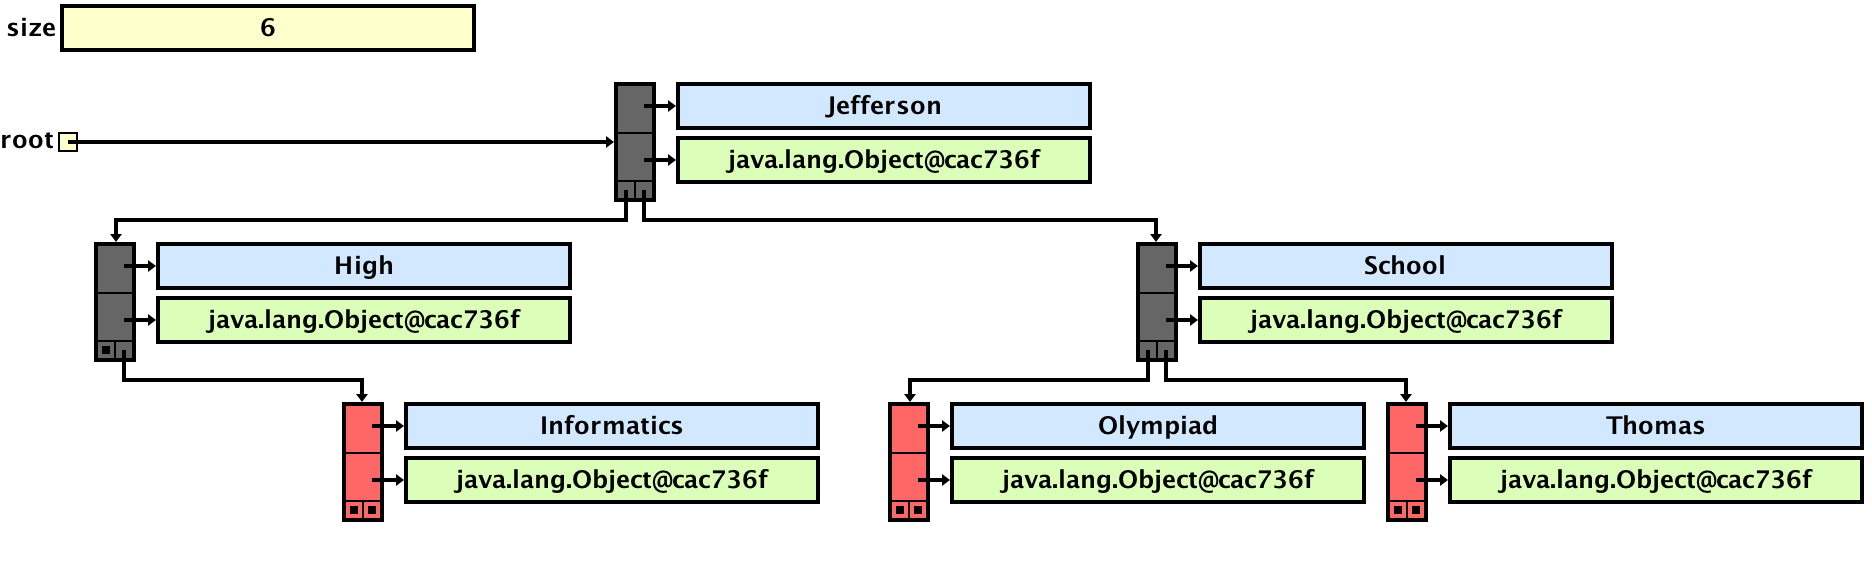
\includegraphics[scale=0.5]{treeset.png}


\subsection{Unordered sets}

In many cases, however, we may actually want to use an unordered set instead. Why? Because while $O(\log n)$ time is pretty good, a \textbf{hash table} can do even better, implementing the same operations in $O(1)$ amortized time!

Hash tables work by computing a \textit{hash}, an integer value produced by a \textit{hash function} based on the value of an item. This hash is then converted to an index in an array, where the item is stored. One major complication is dealing with \textit{collisions}, in which two different items produce the same hash, though we won't discuss how to deal with those here.

Thanks to hashing, however, using an unordered set is nearly as fast as accessing elements in an array, which only takes $O(1)$. As with a dynamic array, however, we occasionally need to expand the size of a hash table, so the actual complexity is again amortized. In the representation below, you can see the hash table for this particular unordered set (notice the collision at index 0).

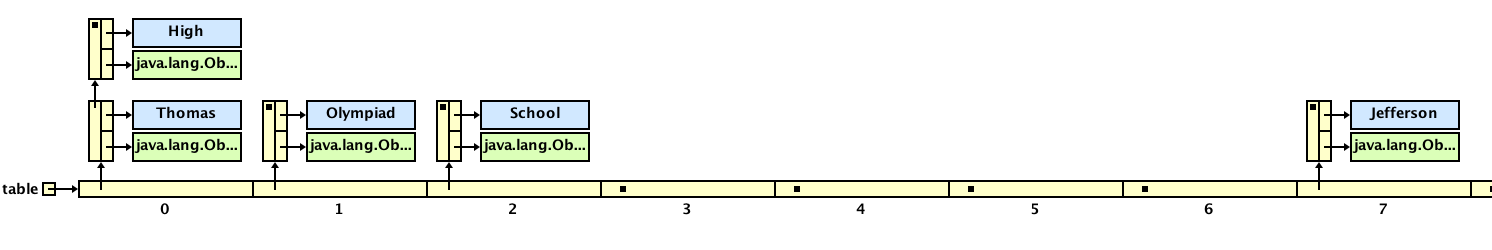
\includegraphics[scale=0.64]{hashset.png} 


